\ifx\mainfile\undefined
%  ========================================================================
%  Copyright (c) 2006-2011 The University of Washington
%
%  Licensed under the Apache License, Version 2.0 (the "License");
%  you may not use this file except in compliance with the License.
%  You may obtain a copy of the License at
%
%      http://www.apache.org/licenses/LICENSE-2.0
%
%  Unless required by applicable law or agreed to in writing, software
%  distributed under the License is distributed on an "AS IS" BASIS,
%  WITHOUT WARRANTIES OR CONDITIONS OF ANY KIND, either express or implied.
%  See the License for the specific language governing permissions and
%  limitations under the License.
%  ========================================================================
%
 
\documentclass [11pt, twoside] {uwthesis}

\usepackage{color}
\usepackage{url}
\usepackage{amsmath}
\usepackage{amsfonts}
\usepackage[bookmarks,
	hidelinks,
	plainpages=false,
	pdfpagelabels,
	pagebackref=true,
            ]{hyperref}
\renewcommand*{\backref}[1]{}% for backref < 1.33 necessary
\renewcommand*{\backrefalt}[4]{%
  \ifcase #1 %
    (No citations.)%
  \or
    (Cited on page #2.)%
  \else
    (Cited on pages #2.)%
  \fi
}

\newcommand{\biburl}[1]{{\tt<}\url{#1}{\tt>}}

\hypersetup{%
pdfauthor = {Daniel Chaim Halperin},
pdftitle = {Simplifying the Configuration of 802.11 Wireless Networks with Effective SNR},
pdfsubject = {Ph.D. Dissertation},
pdfkeywords = {},
pdfcreator = {University of Washington, Computer Science and Engineering},
pdfproducer = {},
bookmarksopen = {true},
pdfpagelayout = {TwoColumnRight},
}

\usepackage{footnotebackref}
%%%%%%%%%%%%%%%%%%%%%%%%%%%%%%%%%%%%%%%%%%%%%%%%%%%%%%
%%%        Formatting sections                     %%%
%%%%%%%%%%%%%%%%%%%%%%%%%%%%%%%%%%%%%%%%%%%%%%%%%%%%%%
\newcommand{\algref}[1]{Algorithm~\ref{#1}}
\newcommand{\chapref}[1]{Chapter~\ref{#1}}
\renewcommand{\eqref}[1]{Equation~\ref{#1}}
\newcommand{\figref}[1]{Figure~\ref{#1}}
\newcommand{\secref}[1]{\S\ref{#1}}
\newcommand{\tabref}[1]{Table~\ref{#1}}
\newcommand{\heading}[1]{\vspace{4pt}\noindent\textbf{#1}}
\newcommand{\topheading}[1]{\noindent\textbf{#1}}
\newcommand{\noheading}[0]{\vspace{4pt}\noindent}

%%%%%%%%%%%%%%%%%%%%%%%%%%%%%%%%%%%%%%%%%%%%%%%%%%%%%%
%%%        XXX and other warnings                  %%%
%%%%%%%%%%%%%%%%%%%%%%%%%%%%%%%%%%%%%%%%%%%%%%%%%%%%%%
\newcommand{\xxx}[1]{\textit{\color{red}XXX #1}}

%%%%%%%%%%%%%%%%%%%%%%%%%%%%%%%%%%%%%%%%%%%%%%%%%%%%%%
%%%        Units                                   %%%
%%%%%%%%%%%%%%%%%%%%%%%%%%%%%%%%%%%%%%%%%%%%%%%%%%%%%%
\usepackage{xspace}
\newcommand{\unitsep}{\texorpdfstring{\,}{ }}
\def\unit#1{% from: http://www.tex.ac.uk/cgi-bin/texfaq2html?label=csname "Defining a macro from an argument"
  \expandafter\def\csname #1\endcsname{\unitsep\text{#1}\xspace}%
}
\def\varunit#1#2{% from: http://www.tex.ac.uk/cgi-bin/texfaq2html?label=csname "Defining a macro from an argument"
  \expandafter\def\csname #1\endcsname{\unitsep\text{#2}\xspace}%
}
\unit{GHz}
\unit{MHz}
\unit{kHz}
\unit{Gbps}
\unit{Mbps}
\unit{KB}
\unit{dB}
\unit{dBi}
\unit{dBm}
\unit{W}
\unit{mW}
\varunit{uW}{$\mu$W}
\unit{ms}
\varunit{us}{$\mu$s}
\unit{h}
\unit{m}
\unit{s}
\unit{km}
\unit{cm}
\unit{mm}
\varunit{mmsq}{mm$^\text{2}$}
\varunit{insq}{in$^\text{2}$}
\newcommand{\degree}{\ensuremath{^\circ}\xspace}
\newcommand{\degrees}{\degree}
%%%%%%%%%%%%%%%%%%%%%%%%%%%%%%%%%%%%%%%%%%%%%%%%%%%%%%%%%%%%%%%%%%%%%%%%%%%%%%%%%%%%%%
% Euler for math | Palatino for rm | Helvetica for ss | Courier for tt
%
% From: http://www.tug.org/mactex/fonts/LaTeX_Preamble-Font_Choices.html
%%%%%%%%%%%%%%%%%%%%%%%%%%%%%%%%%%%%%%%%%%%%%%%%%%%%%%%%%%%%%%%%%%%%%%%%%%%%%%%%%%%%%%
\renewcommand{\rmdefault}{ppl} % rm
\usepackage[scaled]{helvet} % ss
\usepackage{courier} % tt
\usepackage{eulervm} % a better implementation of the euler package (not in gwTeX)
\normalfont
\usepackage[T1]{fontenc}
%%%%%%%%%%%%%%%%%%%%%%%%%%%%%%%%%%%%%%%%%%%%%%%%%%%%%%%%%%%%%%%%%%%%%%%%%%%%%%%%%%%%%%

%%%%%%%%%%%%%%%%%%%%%%%%%%%%%%%%%%%%%%%%%%%%%%%%%%%%%%
%%%        Figures                                 %%%
%%%%%%%%%%%%%%%%%%%%%%%%%%%%%%%%%%%%%%%%%%%%%%%%%%%%%%
\usepackage{graphicx}
% Caption package both lets you set the spacing between figure and caption
% and also makes the \figref{} point to the right place.
\usepackage[font=bf,aboveskip=6pt,belowskip=-4mm]{caption}
% Allow subfigures, make them bold
\usepackage[bf,BF,small]{subfigure}
% List of figures
\setcounter{lofdepth}{2}  % Print the chapter and sections to the lot

%%%%%%%%%%%%%%%%%%%%%%%%%%%%%%%%%%%%%%%%%%%%%%%%%%%%%%
%%%        Lists with reduced spacing              %%%
%%%%%%%%%%%%%%%%%%%%%%%%%%%%%%%%%%%%%%%%%%%%%%%%%%%%%%
\usepackage{enumitem}

%%%%%%%%%%%%%%%%%%%%%%%%%%%%%%%%%%%%%%%%%%%%%%%%%%%%%%
%%%        Fancy tables                            %%%
%%%%%%%%%%%%%%%%%%%%%%%%%%%%%%%%%%%%%%%%%%%%%%%%%%%%%%
\usepackage{tabulary}
\usepackage{booktabs}

%%%%%%%%%%%%%%%%%%%%%%%%%%%%%%%%%%%%%%%%%%%%%%%%%%%%%%
%%%        Formatting techniques/tools/etc.        %%%
%%%%%%%%%%%%%%%%%%%%%%%%%%%%%%%%%%%%%%%%%%%%%%%%%%%%%%
\newcommand{\term}[1]{\texttt{#1}}

\begin{document}
 
\textpages
\setcounter{chapter}{2} % Set to n-1!
\fi
%%%%%%%%%%%%%%%%%%%%%%%%%%%%%%%%%%

\cleardoublepage
\chapter{Problem and Approach}
\label{chap:problem}
\label{chap:approach}

The problem I study in this thesis is how to inform configuration decisions for wireless networks. I begin this chapter by presenting some of the primary problems in this space. Second, I discuss how we handle these problems today---there are two primary classes of techniques: (1) \emph{probe-based} schemes which use packet reception or loss as a high-level indicator of channel performance, and (2) \emph{SNR-based} schemes which use measurements of the total signal power in a channel to predict packet delivery. Finally, I conclude this chapter by presenting the hypothesis of my research, and my approach to demonstrating it.

%According to the standards makers, one of the intended purposes of the RSSI is ``to aid in link optimization algorithms such as roaming decisions''~\cite[\S 19.9.5.10]{80211}.

%\section{Wireless Configuration Problems}
%In this section, I describe the configuration problems that arise in modern wireless links and wireless networks, made concrete in the context of multi-antenna 802.11n.
%
%%%%%%%%%%%%%%%%%%%%%%%%%%%%%%%%%%%%%%%%%%%%%%%%%%%%%%%%%%%%%%%%%%%%%%%%%%%%%%%%%%%%%%%%%%%%%%%%%%%%%%
\section{Problem: Rate Control for a Single Link}
\begin{figure}[t]
	\centering
	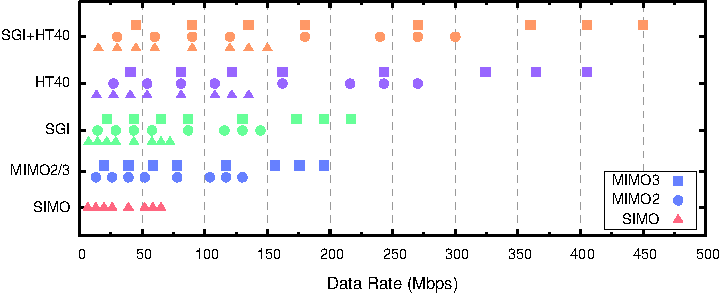
\includegraphics[width=\textwidth]{figures/rate_configs.pdf}
	\caption[The rate-related 802.11n configurations that use three antennas]{\label{fig:rate_configs}The different rate-related 802.11n configurations that use three antennas and 802.11n physical layer enhancements.}
\end{figure}

To accurately choose the rate at which to send data wirelessly, a rate control algorithm must find a good option among many possibilities. With 802.11n, which has adopted modern multi-antenna and physical layer techniques, this problem has gotten significantly more complex. To illustrate this, \figref{fig:rate_configs} shows the available rate configurations in 802.11n for a device with three antennas. These configurations use the eight MCS combinations described in \tabref{tab:siso_mcs}, and the 802.11n enhancements shown in \tabref{tab:11n_enhancements}.

At the bottom of the figure, the SIMO line shows the eight single-stream configurations, which provide rates ranging from 6.5\Mbps to 65\Mbps. These are precisely the eight choices for rate that algorithms controlling a legacy 802.11a/g system must choose from.

In contrast, this space expands by a factor of 12 with 802.11n. Adding a second (MIMO2) and third (MIMO3) spatial stream increases the maximum rate to 195\Mbps, for a total of 24 different configurations. For each of these configurations, 802.11n adds the optional use of double-width (40\MHz, HT40) channels that raises the maximum rate to 405\Mbps with 48 choices. Finally, a physical layer tweak to a shorter OFDM guard interval (SGI) adds another $\approx 11\%$ and pushes the fastest configuration to 450\Mbps among 96 possibilities.

\subsection{Existing Statistics-based Approaches}
\begin{figure}[t]
      \centering
      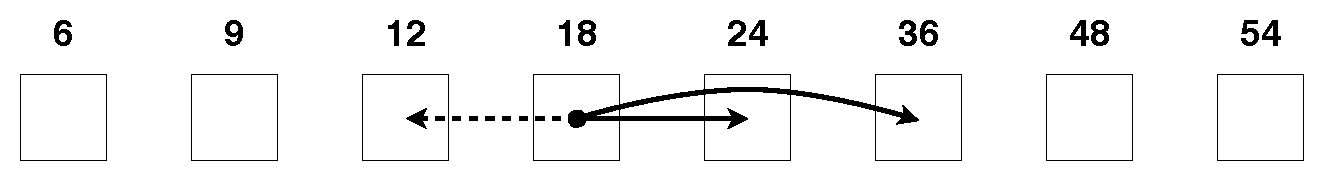
\includegraphics[scale=0.44]{figures/approach_figs/search_11a.pdf}
      \caption[Rate adaptation search pattern for 802.111]{\label{fig:search_11a}A typical rate adaptation search pattern for 802.11a.}
\end{figure}
The majority of rate control algorithms today rely on packet loss statistics to adapt the operating rate. These algorithms use a large number of losses as a signal that the link quality is too poor to support the current rate, and hence fall back to a lower rate that is more easily received. Conversely, when a link experiences a very small number of losses using its current rate, it sends some \emph{packet probes} at a rate, and switches to the faster rate if it also works well. \figref{fig:search_11a} shows a typical 802.11a adaptation search pattern, where each box corresponds to an 802.11a rate and the arrows show the faster (solid) and slower (dashed) rates that might be probed.

The first algorithms (ARF~\cite{Kamerman_ARF} and AARF~\cite{Lacage_AARF}) would only switch between a rate and the next fastest or slowest; later implementations look up to two rates ahead~\cite{Bicket_SampleRate}. Minstrel~\cite{Minstrel}, the dominant 802.11a rate adaptation algorithm used today, performs intelligent (biased) sampling of \emph{all} rates to keep up-to-date estimates of the global rate space and can thus take discontinuous jumps. Recent revisions to these algorithms have focused on better handling of corner cases, such as improving performance during hidden terminals via adaptive control over RTS/CTS~\cite{Minstrel,Wong_RRAA}.

Some algorithms use bit error rate statistics instead of loss rate statistics to adapt rate. SoftRate~\cite{Vutukuru_SoftRate} estimates the bit error rate using a soft-output Viterbi decoder for error correction, and Chen et al.~\cite{Chen_EEC} designed a coding scheme called Error Estimating Coding (EEC) to enable accurate BER estimation at a higher layer.

\subsection{Complication: Multi-dimensional Search Space} 
%The explosion in the sheer number of configurations outlined in the prior section greatly complicates the rate configuration space for 802.11n, however this is only part of the problem.
All of the statistics-based approaches, which walk up or down the list of rates based on whether the current rate works well, implicitly rely on the following basic assumption (outlined by Vutukuru et al.~\cite{Vutukuru_SoftRate}):
\begin{center}
\textbf{Assumption:} \emph{BER is a monotonically increasing function of the bit rate.}
\end{center}
But 802.11n rate configurations are \emph{non-monotonic}. That is, it is not necessarily true that faster configurations are generally less likely to work than slower ones. This violates the axiom of these statistics-based approaches, and hence the \emph{multi-dimensional} search space must be treated as such. I explain why in the following example.

\begin{figure}[t]
      \centering
      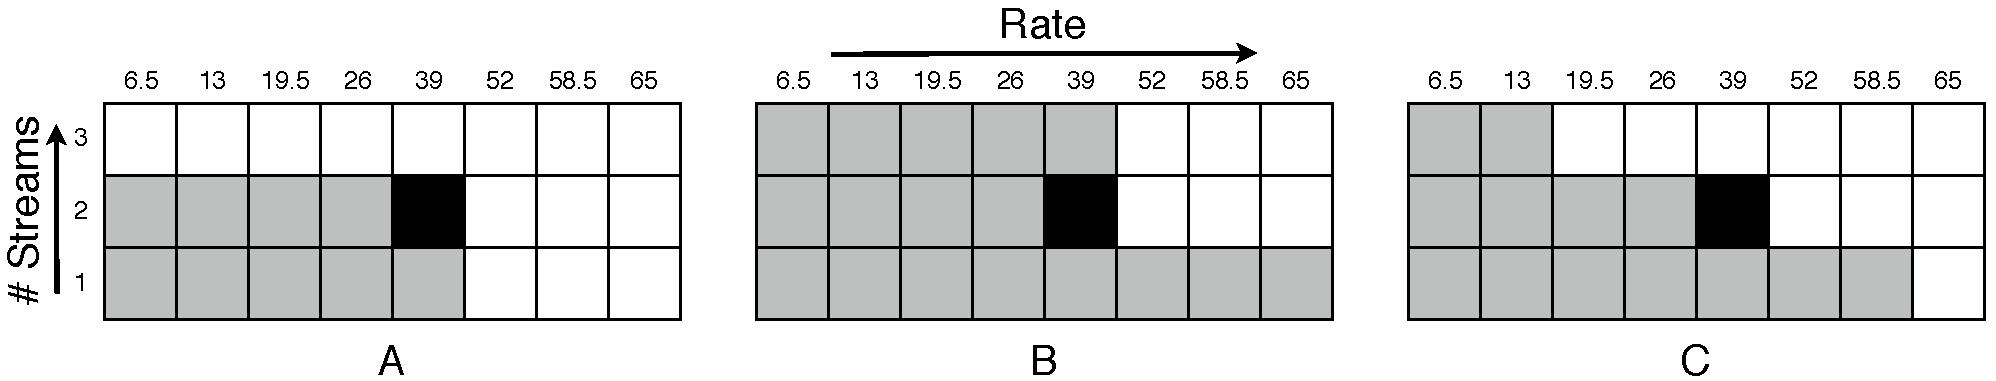
\includegraphics[width=\textwidth]{figures/rate_table_2d.pdf}
      \caption[Three different rate maps for 802.11n links.]{\label{fig:rate_table_2d}Three different rate maps for 802.11n links. On these links, MCS~12 (the black box) is the highest reliable 2-stream rate, and gray boxes indicate other reliable transmit configurations. A (\emph{left}): the worst possible situation in which no 3-stream rates and no higher single-stream configurations work. B (\emph{middle}): the best case in which all single stream rates work and all 3-stream rates work up to 39~Mbps each. C (\emph{right}): an average case in which the set of reliable rates decreases as more spatial streams are used.}
\end{figure}
\begin{figure}[t]
      \centering
      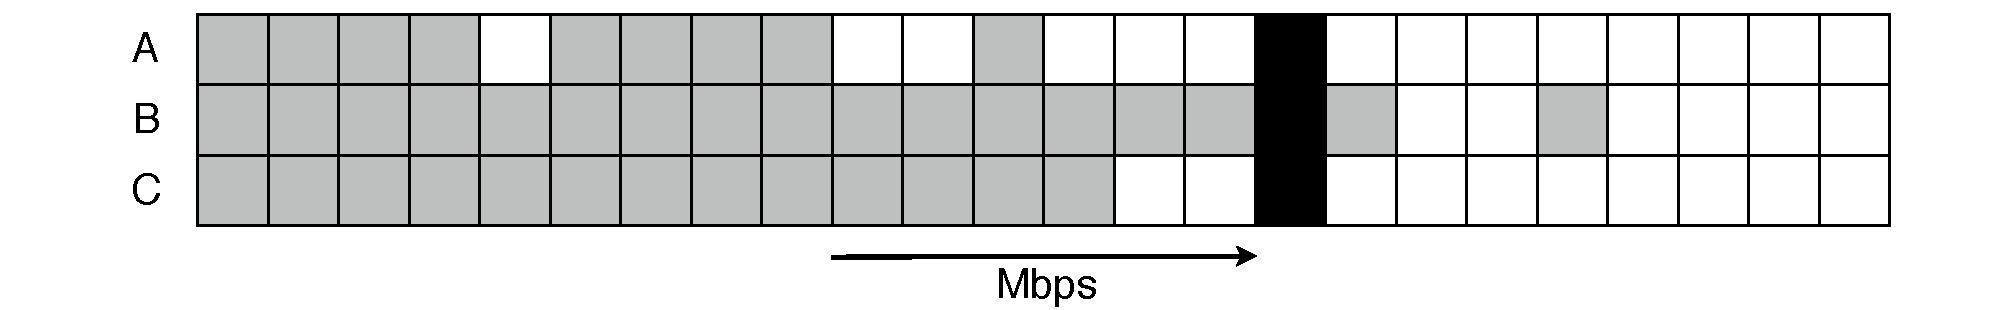
\includegraphics[width=\textwidth]{figures/rate_table_1d.pdf}
      \caption[Rate maps for the links in \figref{fig:rate_table_2d} mapped into one dimension]{\label{fig:rate_table_1d}Rate maps for the links in \figref{fig:rate_table_2d} now mapped into one dimension and sorted by total link speed (Mbps). Ties (e.g., 1x39 and 3x13) are broken such that configurations with fewer streams come first. In this view, the strict monotonicity assumed by rate adaptation algorithms is violated, and the violations occur in a channel-dependent way. Thus, 802.11n rate adaptation requires optimization along multiple dimensions.}
\end{figure}

\figref{fig:rate_table_2d} shows three plausible \define{rate maps} for 3-antenna 802.11n links. In these rate maps, each row represents a different number of spatial streams, and each column represents a different MCS. A cell is shaded if a link can reliably deliver packets using that rate at that number of streams. The black box corresponds to MCS~12---2 streams at 39\Mbps each---which is the highest working 2-stream rate for these three hypothetical links.

In 802.11n, each of the scenarios (A), (B), and (C) illustrated here is possible. In particular, if the link can reliably deliver packets using MCS~12 then it is likely that MCS~4---the same encoding, but fewer streams---works as well. The same holds for MCS~11, since it uses the same number of streams but a less dense encoding. Similar logic implies all the shaded cells in link (A), which represents the most conservative situation in which MCS~12 works well. Conversely, link (B) exhibits the best corresponding situation; higher-encoding single-stream configurations may also deliver most packets, and there may be little penalty from using 3 streams, thus resulting in the same set of 3-stream links working. Finally, link (C) exhibits an average case, in which lower rates must be used as the number of spatial streams increases.

The key is that each of these three links is plausible, which means that the search space for rate is non-monotonic in 802.11n. In \figref{fig:rate_table_1d}, I have redrawn the rate maps for these three links along a single-dimension, sorted by data rate. Ties in pure data rate---e.g., MCS~1 vs MCS~8, both at 13\Mbps---are broken such that fewer streams is lower in the search. Here we can see that for all three links there exist higher rates that work well where lower rates do not. Thus a rate configuration algorithm for a multi-antenna link needs to consider a multi-dimensional search space.

\subsection{Current 802.11n Statistics-based Approaches}
\begin{figure}[t]
      \centering
      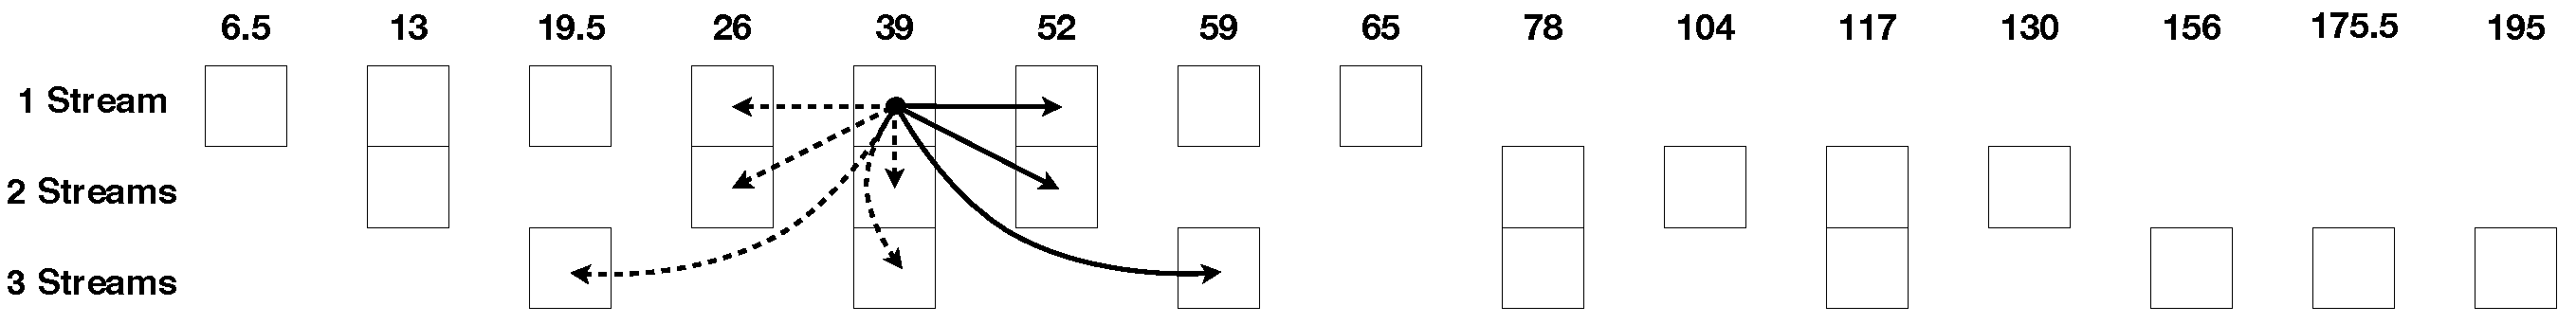
\includegraphics[scale=0.33]{figures/approach_figs/search_11n.pdf}
      \caption[Rate adaptation search pattern for 802.11n]{\label{fig:search_11n}A typical rate adaptation search pattern for 802.11n.}
\end{figure}
\figref{fig:search_11n} illustrates the multi-dimensional search challenge with a concrete example. Each row corresponds to a transmit configuration with one, two, or three spatial streams. The eight boxes correspond to the eight 802.11n MCS combinations, placed in columns that reflect the aggregate link speed.

As we saw in \figref{fig:search_11a}, the single-dimensional search algorithm might try one or two rates higher, and during periods of loss it might fall back to the next lowest rate. In contrast, when increasing 802.11n rate from a single stream at MCS~4 (39\Mbps), the configurations MCS~5 (52\Mbps), MCS~11 (MIMO2-52\Mbps), and MCS~18 (MIMO3-58.5\Mbps) are all transmit configurations with better link speed, and each might work or not work depending on the channel. When MCS~4 experiences loss, there are five choices of fallback configuration. This includes the higher-stream MCS~10 (MIMO2-39\Mbps) and MCS~17 (MIMO3-39\Mbps) which both have the same link speed and might work, as they use more robust modulation and coding combinations.

MiRA~\cite{Pefkianakis_MiRA} is a recent research algorithm that implements a version of this multi-probing scheme, as does the Minstrel\_HT~\cite{Minstrel_HT} algorithm used by the Linux kernel to do 802.11n rate selection in practice. A third approach is used by Intel's iwlwifi driver~\cite{iwlwifi}, which uses an 802.11a-like algorithm to select between configurations that use the same number of streams, and adjusts the number of streams at coarse intervals.

\subsection{State of the Art in Statistics-based Approaches}
The dominant algorithms used in the Linux kernel today are Minstrel~\cite{Minstrel} (for 802.11a/g) and Minstrel\_HT~\cite{Minstrel_HT} (for 802.11n)  In general, statistics-based schemes provide good performance for static links in which the devices do not move and the surrounding environment does not change. For such cases, the algorithms may be inefficient at first but will converge to a good operating point. The challenge, as pointed out by several works~\cite{Holland_RBAR,Judd_CHARM,Vutukuru_SoftRate}, is that---depending on the speed at which devices move or the environment changes---these algorithms may be slow to react to varying conditions in mobile links environments, resulting in significant performance degradation.

SoftRate~\cite{Vutukuru_SoftRate} and EEC~\cite{Chen_EEC} are the newest BER-based adaptation algorithms. Both algorithms provide faster adaptation than their loss-based counterparts because by using the BER they can distinguish between a rate that is barely working with marginal BER (in which case the next fastest rate will not work) or has a lot of headroom (in which case it is worth probing the next fastest rate). These algorithms are effective at shifting up and down within a monotonic rate space; however, their BER estimations do not apply across the orthogonal dimensions such as multiple spatial streams. To handle 802.11n, these algorithms would need to be amended to do multi-dimensional search as well.

%%%%%%%%%%%%%%%%%%%%%%%%%%%%%%%%%%%%%%%%%%%%%%%%%%%%%%%%%%%%%%%%%%%%%%%%%%%%%%%%%%%%%%%%%%%%%%%%%%%%%%
\subsection{SNR-based Approaches}
As I described in \chapref{chap:background} (\figref{fig:mod_ber_snr}), textbook analyses of modulation schemes give delivery probability for a single signal in terms of the signal-to-noise (SNR) ratio~\cite{Goldsmith}.
These theoretical models hold for narrowband channels with additive white Gaussian noise. They predict a sharp transition region of 1--2\dB over which a link changes from extremely lossy to highly reliable. This feature in theory makes the SNR a valuable indicator of performance.

This gives rise to a simple SNR-based configuration scheme, at least for selecting rate: Upon receiving a packet, a device can use the measured RSSI to compute SNR and predict the fastest rate supported. It can then feed this information back to the transmitter, which will use the newly selected rate for subsequent transmissions. This approach was explored in simulation by Holland et al.~\cite{Holland_RBAR} with an algorithm called RBAR, and shown to be effective.

\subsection{Complication: Packet Delivery versus SNR in Practice}
Though SNR-based rate control algorithms may work well in simulation, subsequent practical work found that the SNR computed from RSSI was unreliable~\cite{Aguayo_Roofnet, Reis_interference, Zhao_sensys03}. In very early devices, the RSSI was found to vary wildly over time or device temperature, providing unreliable thresholds; this was corrected by calibration in later devices (e.g., confirmed by Zhang et al.~\cite{Zhang_SNRguided} and by my measurements). Reis et al.~\cite{Reis_interference} found that RSSI estimates were corrupted by interfering transmissions. Finally, even in the absence of these latter effects, several studies found that the same RSSI value gives dramatically different performance for different links.

To understand which effects still hold for 802.11n hardware, I generated performance curves using an Intel Wireless Wi-Fi Link 5300 a/g/n (\program{iwl5300}) wireless network card. I connected two network cards together via a wire, and configured them to operate in a mode that uses a single antenna to transmit or receive. Using an inline variable attenuator I varied the amount of power received, and for each power level I sent around 1,000 packets using each of the eight 802.11n single-stream rates (\tabref{tab:siso_mcs}) and measured the fraction of delivered packets, the \define{packet reception ratio (PRR)}. With these measurements, I plotted the PRR against the link's SNR (computed from RSSI measurements at the receiver), and present the result in \figref{fig:snr_prr_attenuator}. 

\begin{figure}[t!]
	\centering
%	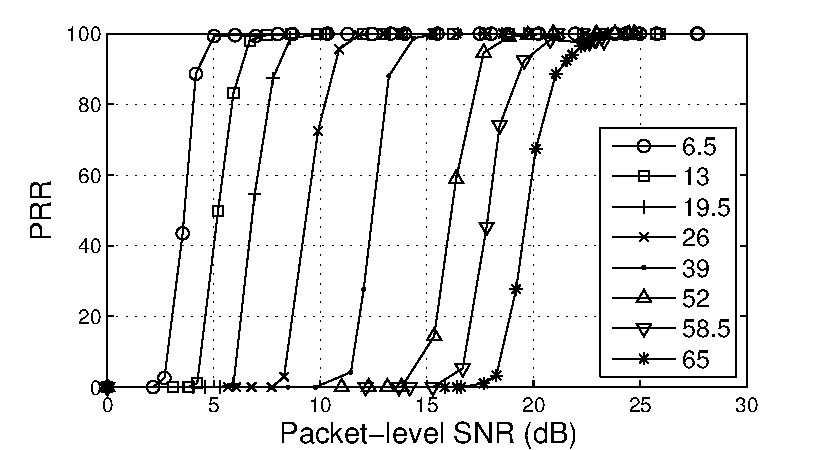
\includegraphics[width=\textwidth,viewport=13 0 364 204,clip]{figures/esnr/embed_attenuator_snr_prr.pdf}
	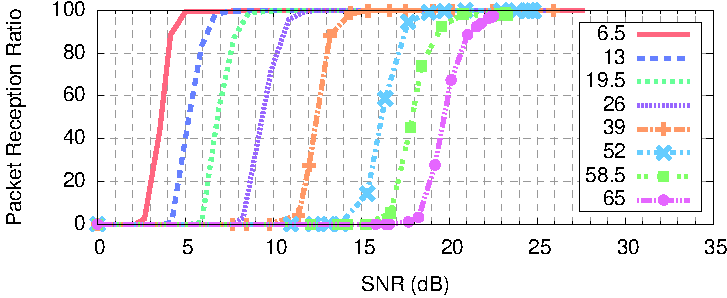
\includegraphics[width=\textwidth]{figures/snr_prr_atten.pdf}
	\caption[SNR vs PRR for a wired 802.11n link]{\label{fig:snr_prr_attenuator}A wired 802.11n link with variable attenuation has a predictable relationship between SNR and packet reception rate (PRR) and clear separation between rates.}
\end{figure}
\begin{figure}[t!]
	\centering
%	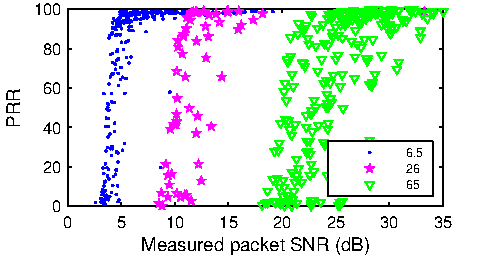
\includegraphics[width=\textwidth,viewport=2 0 217 124,clip]{figures/esnr/embed_scatterplot_meas_snr_small.pdf}
	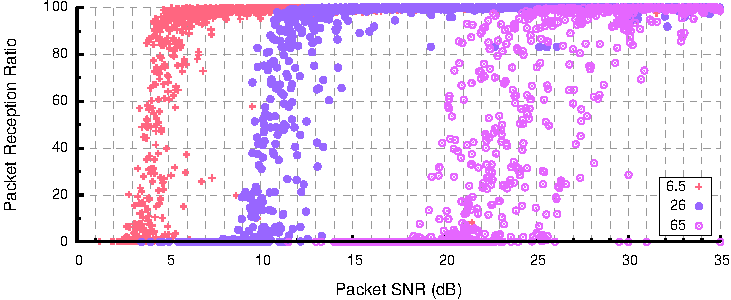
\includegraphics[width=\textwidth]{figures/snr_prr_scatter.pdf}
	\caption[SNR vs PRR for many wireless 802.11n channels]{\label{fig:snr_prr_26_65} Over real wireless channels in our testbeds, the transition region varies by 10\dB or more. The wireless channel loses the clear separation between rates (and so only three rates are shown for legibility).}%
\end{figure}

This figure shows a characteristic sharp transition region between SNR values at which the link goes from lossy to working, 2\dB at low modulations up to 4\dB for the fastest 65\Mbps rate. There is also a clear separation between rates: at a given SNR value, it is clear which rate should be used. This wired link provides a good approximation of a theoretical narrowband channel despite the relatively wide 20\MHz channel, the use of 56 OFDM subcarriers, coding and other bit-level operations. This is the behavior we would want from a link metric in order to predict packet delivery.

In contrast, packet delivery over real wireless channels does not exhibit the same picture. \figref{fig:snr_prr_26_65} shows the measured PRR versus SNR for three sample rates (6.5\Mbps, 26\Mbps, and 65\Mbps) over all wireless links in our testbeds, using the same 802.11n NICs. The SNR of the transition regions can exceed 10\dB, so that some links easily work for a given SNR and others do not. There is no longer clear separation between rates. This is consistent with the measurements from prior work mentioned above~\cite{Aguayo_Roofnet, Judd_CHARM, Reis_interference, Zhang_SNRguided, Zhao_sensys03}.

\subsection{State of the Art in SNR-based Approaches}
Although prior studies and my measurements showed that SNR, based on RSSI, does not accurately predict delivery across links, they also found that for a particular link a higher RSSI generally has higher packet delivery for a given rate~\cite{Aguayo_Roofnet,Judd_CHARM,Zhang_SNRguided}. Consequently, there are two algorithms, SGRA~\cite{Zhang_SNRguided} and CHARM~\cite{Judd_CHARM}, which use SNR feedback from the receiver in conjunction with packet loss statistics in order to learn the relationship between SNR and packet delivery online. Like statistics-based approaches, these algorithms work well for static links. Additionally, they provide good performance for fixed devices in mobile environments~\cite{Judd_CHARM}, because the learned relationship between SNR and PER is only slightly affected by moving objects and the learned calibration is generally valid. Successive measurements by Vutukuru et al.~\cite{Vutukuru_SoftRate} showed that CHARM tended to under-select in mobile links because it was unable to adapt its thresholds quickly enough to respond to the changing channel.

\subsection{Complication: High-level Measurement}
I listed above several reasons that packet-level SNR calculated from RSSI has historically been a poor predictor of performance. In the modern era of calibrated hardware, however, measurements no longer vary significantly with changing temperature or power level, or across devices. Instead, the dominant factor is likely to be the use of OFDM, and the presence of frequency-selective fading in the RF channel. The packet-level SNR, as a measure of the total power in the channel, simply does not reflect the SNRs of the individual subcarriers, and I will show later that this is indeed a major contributor to the inadequacy of RSSI. In the 802.11n use of spatial multiplexing, the receiver takes on SNR value per antenna, now reflecting the total power combined across all spatial streams and all subcarriers. The total power received will vary with the number of streams, and the actual performance of the link will depend on how well this total power is balanced across spatial streams, and how well the receiver can separate the two spatial streams. Thus in 802.11n the RSSI is likely to be even less accurate when predicting link performance.

\subsection{Approach using Low-level RF Measurements}
\label{sec:accurate}
AccuRate~\cite{Sen_AccuRate} takes an alternative approach to using physical layer information to predict performance. Instead of measuring information about the \emph{signal power}, AccuRate measures the \emph{error vectors} (described in \chapref{chap:background}) of the received symbols when demodulating a packet. To make predictions about bit error rate, AccuRate then replays those same error vectors to a physical layer simulator, which models the reception of a packet using each of the different rates and selects the fastest successfully received packet. Though it would be impractical to implement a full physical layer simulator for each received packet, AccuRate was shown to be significantly more accurate than SNR-based algorithms with performance comparable to SoftRate. At the same time, AccuRate suffers from the same 802.11n-related flaws as the remaining algorithms: the magnitude of the error vectors will change depending on different numbers of spatial streams or channel widths or the use of a short guard interval, and AccuRate can handle none of these cases without implementing a multi-dimensional search.

%%%%%%%%%%%%%%%%%%%%%%%%%%%%%%%%%%%%%%%%%%%%%%%%%%%%%%%%%%%%%%%%%%%%%%%%%%%%%%%%%%%%%%%%%%%%%%%%%%%%%%
\section{Further Wireless Configuration Problems}
In the previous section, I outlined the 802.11n rate configuration problem, the current approaches, and the multi-dimensional aspects of 802.11n that make them ineffective. In this section, I briefly mention many other problems and how they are solved in Wi-Fi networks today.

\subsection{Antenna Selection}
Probe. Among production drivers, only Intel~\cite{iwlwifi} does it.
\subsection{Channel Width Selection}
As part of rate adaptation; probe.
\subsection{Transmit Power Control}
Unused in practice. Research?
\subsection{Access Point Selection}
Highest RSS, maybe idle time. Lots of research in AP-based systems, e.g., DAIR.
\subsection{Channel Selection}
Irrelevant to today's AP networks, except that APs might switch channel occasionally if interference.
\subsection{Multi-Hop Routing}
Irrelevant to today's AP networks. State of the art is Bahl et al.~\cite{Bahl_repeater} which uses SNR based on RSSI to predict Mbps and then uses that.
\subsection{Spatial Reuse}
Adaptive use of RTS/CTS to prevent it from happening. State of the art is CMAP~\cite{Vutukuru_CMAP} which used fixed entire network to the same rate and still required very complex probing algorithm.
\subsection{Beamforming}
Today, unused. Intel's hardware: does SVD-based beamforming.

%%%%%%%%%%%%%%%%%%%%%%%%%%%%%%%%%%%%%%%%%%%%%%%%%%%%%%%%%%%%%%%%%%%%%%%%%%%%%%%%%%%%%%%%%%%%%%%%%%%%%%
\section{My Approach}
My hypothesis is that physical layer measurements can indeed be useful indicators of wireless link performance in practice---even with modern advances at the physical layer---and that these measurements can be used to inform a wide array of link and network configuration problems. My approach to resolving this hypothesis is to build a system that demonstrates that this is true.

In particular, I develop a practical methodology that uses this information and the concept of an effective SNR~\cite{Nanda_EffectiveSNR} to predict performance for wireless channels that use modern physical layer technologies such as OFDM, multiple antennas, variable channel widths, and spatial diversity and multiplexing. I also explain how to apply this prediction engine to a wide variety of link and network configuration problems such as those described in this section. To demonstrate that this methodology is practical, I prototype a working system in the context of IEEE 802.11n, which is the dominant consumer wireless networking technology today and includes these state-of-the-art RF techniques. Finally, to show that it works, I use my prototype to evaluate the accuracy of the choices made using my techniques. I find that my model accurately predicts packet delivery over hundreds of indoor wireless links in two environments, and that this level of accuracy is sufficient to lead to good configurations for many link and network problems.

\begin{figure}[t]
  \centering
%  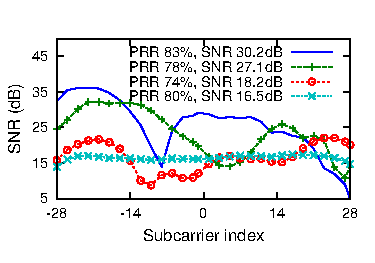
\includegraphics[width=\columnwidth,viewport=2 9 185 108,clip]{figures/esnr/embed_fsf-shape-two-links.pdf}
  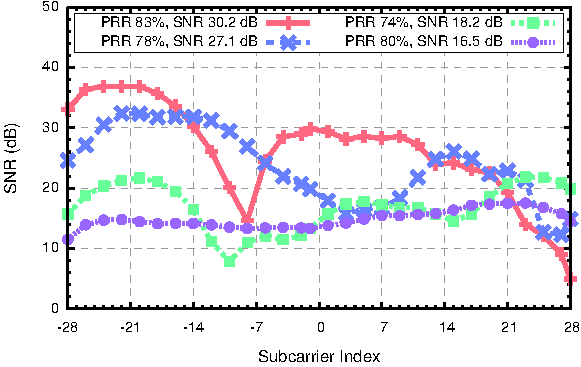
\includegraphics[width=0.8\textwidth]{figures/fsf_shape.pdf}
  \caption[Channel gains on four links that perform about equally well at 52\Mbps.]{Channel gains on four links that perform about equally well at 52\Mbps. The more faded links require larger RSSIs (i.e., more transmit power) to achieve similar PRRs.}
  \label{fig:example_fsf_shape}
  % information for the links used to make above plot: 
  %srcs = [1 10 3 3];
  %dests = [9 11 2 5];
  %txpowers = [-4 20 28 20];

  % reference numbers from expt-8
  %prr = [80 83 78 74];
  %rss = [16.5 30.2 27.1 18.2];
\end{figure}

\subsection{Fine-grained RF Measurements}
In this thesis, I claim that low-level measurements of the RF channel can be used to gain insight into the factors that truly determine link performance. To illustrate this fact, I chose four representative links in my 802.11n testbed. These four links have SNRs ranging from 16\dB to 30\dB and yet they each perform similarly, delivering around 80\% of packets sent using single-stream MCS~6 (52\Mbps). \figref{fig:example_fsf_shape} shows the packet reception rates and SNRs for these four links, but also includes the SNRs of the individual OFDM subcarriers for each links.

With this detailed picture, we can see that multipath causes some subcarriers to work markedly better than others although all use the same modulation and coding. These channel details, and not simply the overall signal strength as given by SNR, affect packet delivery. The fading profiles vary significantly across the four links. One distribution is quite flat across the subcarriers, while the other three exhibit frequency-selective fading of varying degrees. Two of the links have two deeply-faded subcarriers that are more than 20\dB down from the peak.

Because of these different fading profiles, these links harness the received power with different efficiencies.
The more faded links are more likely to have errors that must be repaired with coding, and require extra transmit power to compensate. Thus, while the performance is roughly the same, the most frequency-selective link needs a much higher overall packet SNR~(30.2\dB) than the frequency-flat link~(16.5\dB). This difference of almost 14\dB (more than $20\times$) highlights why RSSI-based SNR does not reliably predict performance.
%Fading and its effects are well-known. However, it is rare to see data that shows fading for real links and NICs because it has been difficult to measure.

This example indicates that fine-grained RF measurements can help explain performance for real wireless links. The particular detailed measurements I use this this thesis are called Channel State Information (CSI). For an OFDM link, the CSI comprises the channel gain coefficient (amplitude and phase,\footnote{Note that in \figref{fig:example_fsf_shape}, I plot only the amplitude as the phase offset does not affect packet delivery for a SISO link (assuming it is properly equalized by the receiver).} see \chapref{chap:background}) for each OFDM subcarrier. For an $N$x$M$ MIMO link, the CSI is an $N$x$M$ matrix where each entry reflects the channel gain coefficient from one transmit antenna to one receive antenna. For a MIMO-OFDM link such as in 802.11n, the CSI comprises a three-dimensional $N$x$M$x$S$ matrix that reflects the $N$x$M$ MIMO link for each of $S$ subcarriers.

\subsection{Effective SNR-based Model}
\begin{figure}[t!]
	\centering
	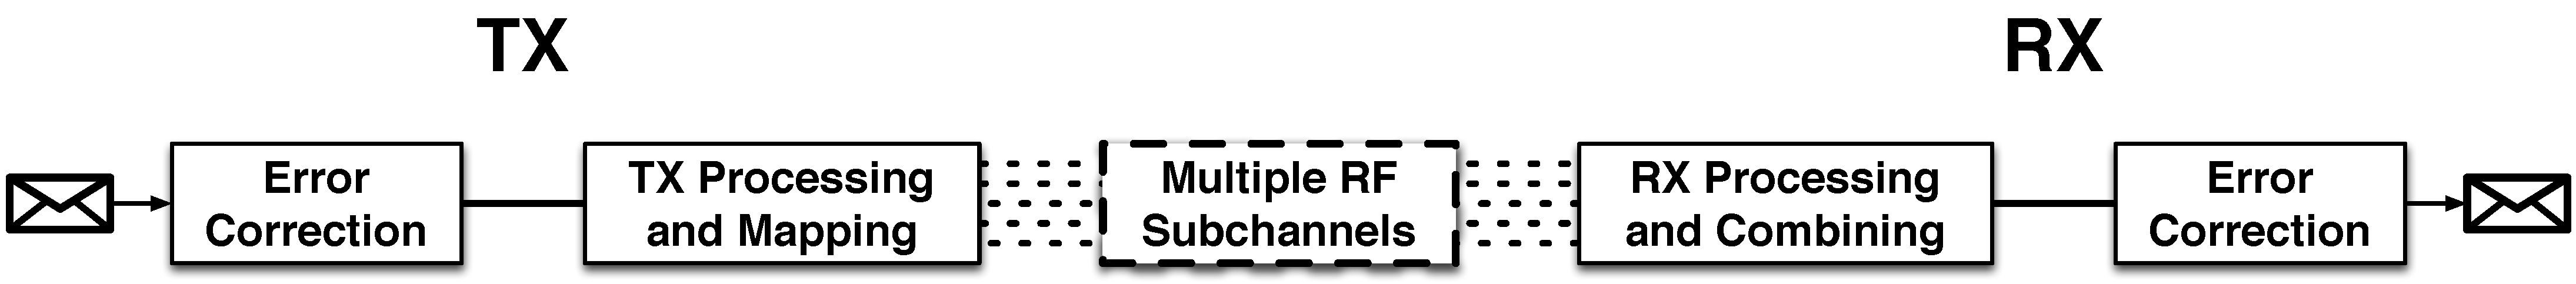
\includegraphics[width=\textwidth]{figures/esnr_intuitive.pdf}
	\caption{\label{fig:esnr_intuitive}Simplified overview of an RF link operating over multiple subchannels.}
\end{figure}

The example of \figref{fig:example_fsf_shape} indicated that the extra information in CSI can help explain performance for real wireless links, though I have not yet established a method to do so. The central component in my thesis is a model for packet delivery that uses CSI to predict packet loss over real wireless channels. To be useful, this model must accurately predict the packet delivery probability for a given physical layer configuration operating over a given channel. It must also simple and practical, so that it can be readily deployed, and cover a wide range of physical layer configurations, so that it can be applied in many settings and for many tasks.

In this thesis, I scope my model to devices that use MIMO and OFDM, which captures the fundamental technological primitives for many current and future networks. In particular, the scope of my model is 802.11n including all the enhancements described in \secref{sec:background_80211n}. My model is based on the concept of Effective $E_b/N_0$ developed by Nanda and Rege~\cite{Nanda_EffectiveSNR}, and described as follows.
 
\figref{fig:esnr_intuitive} shows a simplified overview of a link operating over an RF channel that has multiple subchannels, such as MIMO spatial paths or OFDM subcarriers. The transmitter applies error correction to the original data packet, and then processes the coded bitstream and maps the resulting symbols onto the multiple subchannels. The receiver processes the noisy signal and to recover the (potentially errored) coded bitstream, and then uses error correction to attempt to recover the original data bits. The key hypothesis introduced by Nanda and Rege, is that error correction---in conjunction with mechanisms like frequency- and spatial-aware interleaving in 802.11n---works to spread the errors caused by faded subchannels across the entire channel. If this assumption holds, the link can be modeled as performing with an aggregate error rate equal to the average error rate across subchannels. This average bit error rate is called the \define{Effective BER} of the channel, and from it we can compute the \define{Effective SNR} of the channel. Since the four links displayed in \figref{fig:example_fsf_shape} have similar error performance, they should have similar Effective SNRs. Then the Effective SNR can be used as a metric of link quality, and hence provide accurate estimates of packet delivery.

The model is described in complete detail in the next chapter, but the basic structure of the model is simple: given (1) a current CSI measurement of the RF channel between transmitter and receiver, and (2) a target physical layer configuration of the transmit and receive NICs, it predicts whether that link will reliably deliver packets in that configuration. I do not try to make predictions in the transition region during which a link changes from lossy to reliable. Predictions there are likely to be variable, and simply knowing when the link starts to work is useful information in practice. For the model output, I define that the link will work, i.e., will reliably deliver packets, if the model predicts $\geq$90\% packet reception rate.

With this simple decision primitive, we can easily build higher layer optimization protocols. These include solutions to all of the problems mentioned in this chapter, such as selecting the best rate, number of spatial streams, or transmit antenna set; whether to use 20\MHz or the entire 40\MHz channel; or choosing the lowest transmit power at which the link supports a particular rate. In the next chapter I describe the model and how to use it to solve these problems.

%steps are (1) comprehensively measuring CSI for the RF channel including all subchannels, (2) adapting that CSI measurement to model the transmit configuration problem under investigation, (3) modeling receiver behavior to come up with the post-processing SNRs of the individual subchannels, and (4) computing the bit error rates of the individual subchannels from their SNRs and then calculating the Effective BER and finally the Effective SNR.



%%%%%%%%%%%%%%%%%%%%%%%%%%%%%%%%%%
\ifx\mainfile\undefined
%
% ==========   Bibliography   ==========
%
%\nocite{*}   % include everything in the uwthesis.bib file
\bibliographystyle{plain}
\bibliography{dhalperi_thesis}

\end{document}
\fi
